\documentclass[1p]{elsarticle_modified}
%\bibliographystyle{elsarticle-num}

%\usepackage[colorlinks]{hyperref}
%\usepackage{abbrmath_seonhwa} %\Abb, \Ascr, \Acal ,\Abf, \Afrak
\usepackage{amsfonts}
\usepackage{amssymb}
\usepackage{amsmath}
\usepackage{amsthm}
\usepackage{scalefnt}
\usepackage{amsbsy}
\usepackage{kotex}
\usepackage{caption}
\usepackage{subfig}
\usepackage{color}
\usepackage{graphicx}
\usepackage{xcolor} %% white, black, red, green, blue, cyan, magenta, yellow
\usepackage{float}
\usepackage{setspace}
\usepackage{hyperref}

\usepackage{tikz}
\usetikzlibrary{arrows}

\usepackage{multirow}
\usepackage{array} % fixed length table
\usepackage{hhline}

%%%%%%%%%%%%%%%%%%%%%
\makeatletter
\renewcommand*\env@matrix[1][\arraystretch]{%
	\edef\arraystretch{#1}%
	\hskip -\arraycolsep
	\let\@ifnextchar\new@ifnextchar
	\array{*\c@MaxMatrixCols c}}
\makeatother %https://tex.stackexchange.com/questions/14071/how-can-i-increase-the-line-spacing-in-a-matrix
%%%%%%%%%%%%%%%

\usepackage[normalem]{ulem}

\newcommand{\msout}[1]{\ifmmode\text{\sout{\ensuremath{#1}}}\else\sout{#1}\fi}
%SOURCE: \msout is \stkout macro in https://tex.stackexchange.com/questions/20609/strikeout-in-math-mode

\newcommand{\cancel}[1]{
	\ifmmode
	{\color{red}\msout{#1}}
	\else
	{\color{red}\sout{#1}}
	\fi
}

\newcommand{\add}[1]{
	{\color{blue}\uwave{#1}}
}

\newcommand{\replace}[2]{
	\ifmmode
	{\color{red}\msout{#1}}{\color{blue}\uwave{#2}}
	\else
	{\color{red}\sout{#1}}{\color{blue}\uwave{#2}}
	\fi
}

\newcommand{\Sol}{\mathcal{S}} %segment
\newcommand{\D}{D} %diagram
\newcommand{\A}{\mathcal{A}} %arc


%%%%%%%%%%%%%%%%%%%%%%%%%%%%%5 test

\def\sl{\operatorname{\textup{SL}}(2,\Cbb)}
\def\psl{\operatorname{\textup{PSL}}(2,\Cbb)}
\def\quan{\mkern 1mu \triangleright \mkern 1mu}

\theoremstyle{definition}
\newtheorem{thm}{Theorem}[section]
\newtheorem{prop}[thm]{Proposition}
\newtheorem{lem}[thm]{Lemma}
\newtheorem{ques}[thm]{Question}
\newtheorem{cor}[thm]{Corollary}
\newtheorem{defn}[thm]{Definition}
\newtheorem{exam}[thm]{Example}
\newtheorem{rmk}[thm]{Remark}
\newtheorem{alg}[thm]{Algorithm}

\newcommand{\I}{\sqrt{-1}}
\begin{document}

%\begin{frontmatter}
%
%\title{Boundary parabolic representations of knots up to 8 crossings}
%
%%% Group authors per affiliation:
%\author{Yunhi Cho} 
%\address{Department of Mathematics, University of Seoul, Seoul, Korea}
%\ead{yhcho@uos.ac.kr}
%
%
%\author{Seonhwa Kim} %\fnref{s_kim}}
%\address{Center for Geometry and Physics, Institute for Basic Science, Pohang, 37673, Korea}
%\ead{ryeona17@ibs.re.kr}
%
%\author{Hyuk Kim}
%\address{Department of Mathematical Sciences, Seoul National University, Seoul 08826, Korea}
%\ead{hyukkim@snu.ac.kr}
%
%\author{Seokbeom Yoon}
%\address{Department of Mathematical Sciences, Seoul National University, Seoul, 08826,  Korea}
%\ead{sbyoon15@snu.ac.kr}
%
%\begin{abstract}
%We find all boundary parabolic representation of knots up to 8 crossings.
%
%\end{abstract}
%\begin{keyword}
%    \MSC[2010] 57M25 
%\end{keyword}
%
%\end{frontmatter}

%\linenumbers
%\tableofcontents
%
\newcommand\colored[1]{\textcolor{white}{\rule[-0.35ex]{0.8em}{1.4ex}}\kern-0.8em\color{red} #1}%
%\newcommand\colored[1]{\textcolor{white}{ #1}\kern-2.17ex	\textcolor{white}{ #1}\kern-1.81ex	\textcolor{white}{ #1}\kern-2.15ex\color{red}#1	}

{\Large $\underline{12n_{0758}~(K12n_{0758})}$}

\setlength{\tabcolsep}{10pt}
\renewcommand{\arraystretch}{1.6}
\vspace{1cm}\begin{tabular}{m{100pt}>{\centering\arraybackslash}m{274pt}}
\multirow{5}{120pt}{
	\centering
	\includegraphics[width=112pt]{../../../GIT/diagram.site/Diagrams/png/2847_12n_0758.png}\\
\ \ \ A knot diagram\footnotemark}&
\allowdisplaybreaks
\textbf{Linearized knot diagam} \\
\cline{2-2}
 &
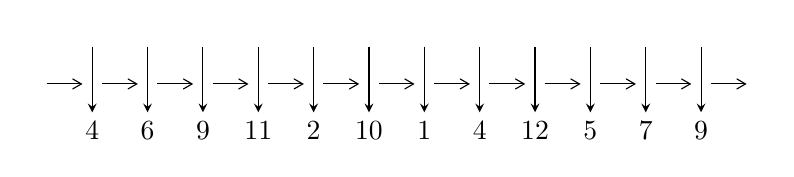
\begin{tikzpicture}[x=20pt, y=17pt]
	% nodes
	\node (C0) at (0, 0) {};
	\node (C1) at (1, 0) {};
	\node (C1U) at (1, +1) {};
	\node (C1D) at (1, -1) {4};

	\node (C2) at (2, 0) {};
	\node (C2U) at (2, +1) {};
	\node (C2D) at (2, -1) {6};

	\node (C3) at (3, 0) {};
	\node (C3U) at (3, +1) {};
	\node (C3D) at (3, -1) {9};

	\node (C4) at (4, 0) {};
	\node (C4U) at (4, +1) {};
	\node (C4D) at (4, -1) {11};

	\node (C5) at (5, 0) {};
	\node (C5U) at (5, +1) {};
	\node (C5D) at (5, -1) {2};

	\node (C6) at (6, 0) {};
	\node (C6U) at (6, +1) {};
	\node (C6D) at (6, -1) {10};

	\node (C7) at (7, 0) {};
	\node (C7U) at (7, +1) {};
	\node (C7D) at (7, -1) {1};

	\node (C8) at (8, 0) {};
	\node (C8U) at (8, +1) {};
	\node (C8D) at (8, -1) {4};

	\node (C9) at (9, 0) {};
	\node (C9U) at (9, +1) {};
	\node (C9D) at (9, -1) {12};

	\node (C10) at (10, 0) {};
	\node (C10U) at (10, +1) {};
	\node (C10D) at (10, -1) {5};

	\node (C11) at (11, 0) {};
	\node (C11U) at (11, +1) {};
	\node (C11D) at (11, -1) {7};

	\node (C12) at (12, 0) {};
	\node (C12U) at (12, +1) {};
	\node (C12D) at (12, -1) {9};
	\node (C13) at (13, 0) {};

	% arrows
	\draw[->,>={angle 60}]
	(C0) edge (C1) (C1) edge (C2) (C2) edge (C3) (C3) edge (C4) (C4) edge (C5) (C5) edge (C6) (C6) edge (C7) (C7) edge (C8) (C8) edge (C9) (C9) edge (C10) (C10) edge (C11) (C11) edge (C12) (C12) edge (C13) ;	\draw[->,>=stealth]
	(C1U) edge (C1D) (C2U) edge (C2D) (C3U) edge (C3D) (C4U) edge (C4D) (C5U) edge (C5D) (C6U) edge (C6D) (C7U) edge (C7D) (C8U) edge (C8D) (C9U) edge (C9D) (C10U) edge (C10D) (C11U) edge (C11D) (C12U) edge (C12D) ;
	\end{tikzpicture} \\
\hhline{~~} \\& 
\textbf{Solving Sequence} \\ \cline{2-2} 
 &
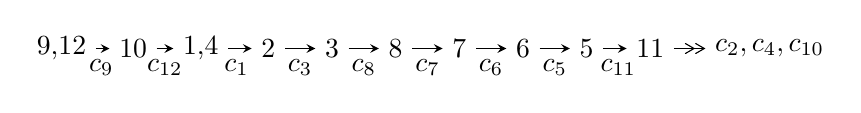
\begin{tikzpicture}[x=23pt, y=7pt]
	% node
	\node (A0) at (-1/8, 0) {9,12};
	\node (A1) at (1, 0) {10};
	\node (A2) at (33/16, 0) {1,4};
	\node (A3) at (25/8, 0) {2};
	\node (A4) at (33/8, 0) {3};
	\node (A5) at (41/8, 0) {8};
	\node (A6) at (49/8, 0) {7};
	\node (A7) at (57/8, 0) {6};
	\node (A8) at (65/8, 0) {5};
	\node (A9) at (73/8, 0) {11};
	\node (C1) at (1/2, -1) {$c_{9}$};
	\node (C2) at (3/2, -1) {$c_{12}$};
	\node (C3) at (21/8, -1) {$c_{1}$};
	\node (C4) at (29/8, -1) {$c_{3}$};
	\node (C5) at (37/8, -1) {$c_{8}$};
	\node (C6) at (45/8, -1) {$c_{7}$};
	\node (C7) at (53/8, -1) {$c_{6}$};
	\node (C8) at (61/8, -1) {$c_{5}$};
	\node (C9) at (69/8, -1) {$c_{11}$};
	\node (A10) at (11, 0) {$c_{2},c_{4},c_{10}$};

	% edge
	\draw[->,>=stealth]	
	(A0) edge (A1) (A1) edge (A2) (A2) edge (A3) (A3) edge (A4) (A4) edge (A5) (A5) edge (A6) (A6) edge (A7) (A7) edge (A8) (A8) edge (A9) ;
	\draw[->>,>={angle 60}]	
	(A9) edge (A10);
\end{tikzpicture} \\ 

\end{tabular} \\

\footnotetext{
The image of knot diagram is generated by the software ``\textbf{Draw programme}" developed by Andrew Bartholomew(\url{http://www.layer8.co.uk/maths/draw/index.htm\#Running-draw}), where we modified some parts for our purpose(\url{https://github.com/CATsTAILs/LinksPainter}).
}\phantom \\ \newline 
\centering \textbf{Ideals for irreducible components\footnotemark of $X_{\text{par}}$} 
 
\begin{align*}
I^u_{1}&=\langle 
8.72942\times10^{279} u^{83}-3.70180\times10^{280} u^{82}+\cdots+2.19369\times10^{283} b+5.24856\times10^{283},\\
\phantom{I^u_{1}}&\phantom{= \langle  }-1.73871\times10^{284} u^{83}+3.54688\times10^{284} u^{82}+\cdots+8.62121\times10^{285} a+9.41097\times10^{286},\\
\phantom{I^u_{1}}&\phantom{= \langle  }u^{84}-2 u^{83}+\cdots-931 u+393\rangle \\
I^u_{2}&=\langle 
5.19189\times10^{21} u^{32}-9.68160\times10^{21} u^{31}+\cdots+1.69614\times10^{22} b-1.88611\times10^{23},\\
\phantom{I^u_{2}}&\phantom{= \langle  }9.63063\times10^{21} u^{32}-6.63604\times10^{22} u^{31}+\cdots+2.66537\times10^{22} a+9.17471\times10^{23},\;u^{33}-3 u^{32}+\cdots-3 u-11\rangle \\
\\
\end{align*}
\raggedright * 2 irreducible components of $\dim_{\mathbb{C}}=0$, with total 117 representations.\\
\footnotetext{All coefficients of polynomials are rational numbers. But the coefficients are sometimes approximated in decimal forms when there is not enough margin.}
\newpage
\renewcommand{\arraystretch}{1}
\centering \section*{I. $I^u_{1}= \langle 8.73\times10^{279} u^{83}-3.70\times10^{280} u^{82}+\cdots+2.19\times10^{283} b+5.25\times10^{283},\;-1.74\times10^{284} u^{83}+3.55\times10^{284} u^{82}+\cdots+8.62\times10^{285} a+9.41\times10^{286},\;u^{84}-2 u^{83}+\cdots-931 u+393 \rangle$}
\flushleft \textbf{(i) Arc colorings}\\
\begin{tabular}{m{7pt} m{180pt} m{7pt} m{180pt} }
\flushright $a_{9}=$&$\begin{pmatrix}1\\0\end{pmatrix}$ \\
\flushright $a_{12}=$&$\begin{pmatrix}0\\u\end{pmatrix}$ \\
\flushright $a_{10}=$&$\begin{pmatrix}1\\u^2\end{pmatrix}$ \\
\flushright $a_{1}=$&$\begin{pmatrix}- u\\u\end{pmatrix}$ \\
\flushright $a_{4}=$&$\begin{pmatrix}0.0201678 u^{83}-0.0411413 u^{82}+\cdots+37.2561 u-10.9161\\-0.000397933 u^{83}+0.00168747 u^{82}+\cdots-1.39648 u-2.39257\end{pmatrix}$ \\
\flushright $a_{2}=$&$\begin{pmatrix}0.0161633 u^{83}-0.0261933 u^{82}+\cdots+26.1042 u-11.4528\\0.00781208 u^{83}-0.0178962 u^{82}+\cdots+12.4153 u-7.75229\end{pmatrix}$ \\
\flushright $a_{3}=$&$\begin{pmatrix}0.0197698 u^{83}-0.0394538 u^{82}+\cdots+35.8597 u-13.3086\\-0.000397933 u^{83}+0.00168747 u^{82}+\cdots-1.39648 u-2.39257\end{pmatrix}$ \\
\flushright $a_{8}=$&$\begin{pmatrix}0.0206064 u^{83}-0.0260386 u^{82}+\cdots+19.3445 u+2.04760\\-0.000880470 u^{83}-0.00560114 u^{82}+\cdots+7.71886 u-7.99711\end{pmatrix}$ \\
\flushright $a_{7}=$&$\begin{pmatrix}0.0183344 u^{83}-0.0267967 u^{82}+\cdots+18.8652 u-1.02254\\0.00139156 u^{83}-0.00484311 u^{82}+\cdots+8.19811 u-4.92696\end{pmatrix}$ \\
\flushright $a_{6}=$&$\begin{pmatrix}0.0219774 u^{83}-0.0304770 u^{82}+\cdots+25.0778 u-2.06978\\0.00306746 u^{83}-0.00998246 u^{82}+\cdots+10.1234 u-6.34404\end{pmatrix}$ \\
\flushright $a_{5}=$&$\begin{pmatrix}0.0249425 u^{83}-0.0285448 u^{82}+\cdots+18.3761 u+11.2314\\-0.00242622 u^{83}+0.0000518733 u^{82}+\cdots+7.71179 u-4.90936\end{pmatrix}$ \\
\flushright $a_{11}=$&$\begin{pmatrix}-0.0267748 u^{83}+0.0522669 u^{82}+\cdots-49.2862 u+13.0525\\0.00829693 u^{83}-0.0131191 u^{82}+\cdots+8.72583 u+0.990108\end{pmatrix}$\\&\end{tabular}
\flushleft \textbf{(ii) Obstruction class $= -1$}\\~\\
\flushleft \textbf{(iii) Cusp Shapes $= 0.0195060 u^{83}-0.0235693 u^{82}+\cdots+27.4576 u-11.4055$}\\~\\
\newpage\renewcommand{\arraystretch}{1}
\flushleft \textbf{(iv) u-Polynomials at the component}\newline \\
\begin{tabular}{m{50pt}|m{274pt}}
Crossings & \hspace{64pt}u-Polynomials at each crossing \\
\hline $$\begin{aligned}c_{1}\end{aligned}$$&$\begin{aligned}
&u^{84}-3 u^{83}+\cdots+8464 u+8464
\end{aligned}$\\
\hline $$\begin{aligned}c_{2},c_{5}\end{aligned}$$&$\begin{aligned}
&u^{84}+4 u^{83}+\cdots-959 u-69
\end{aligned}$\\
\hline $$\begin{aligned}c_{3},c_{8}\end{aligned}$$&$\begin{aligned}
&u^{84}- u^{83}+\cdots-231109 u-59333
\end{aligned}$\\
\hline $$\begin{aligned}c_{4},c_{10}\end{aligned}$$&$\begin{aligned}
&u^{84}- u^{83}+\cdots-99 u-85
\end{aligned}$\\
\hline $$\begin{aligned}c_{6}\end{aligned}$$&$\begin{aligned}
&u^{84}+8 u^{83}+\cdots+13309 u+799
\end{aligned}$\\
\hline $$\begin{aligned}c_{7}\end{aligned}$$&$\begin{aligned}
&u^{84}+2 u^{83}+\cdots-28656216 u-9025047
\end{aligned}$\\
\hline $$\begin{aligned}c_{9},c_{12}\end{aligned}$$&$\begin{aligned}
&u^{84}-2 u^{83}+\cdots-931 u+393
\end{aligned}$\\
\hline $$\begin{aligned}c_{11}\end{aligned}$$&$\begin{aligned}
&u^{84}-2 u^{83}+\cdots-66 u-71
\end{aligned}$\\
\hline
\end{tabular}\\~\\
\newpage\renewcommand{\arraystretch}{1}
\flushleft \textbf{(v) Riley Polynomials at the component}\newline \\
\begin{tabular}{m{50pt}|m{274pt}}
Crossings & \hspace{64pt}Riley Polynomials at each crossing \\
\hline $$\begin{aligned}c_{1}\end{aligned}$$&$\begin{aligned}
&y^{84}-105 y^{83}+\cdots-4667929856 y+71639296
\end{aligned}$\\
\hline $$\begin{aligned}c_{2},c_{5}\end{aligned}$$&$\begin{aligned}
&y^{84}-54 y^{83}+\cdots-314551 y+4761
\end{aligned}$\\
\hline $$\begin{aligned}c_{3},c_{8}\end{aligned}$$&$\begin{aligned}
&y^{84}-91 y^{83}+\cdots-79247924731 y+3520404889
\end{aligned}$\\
\hline $$\begin{aligned}c_{4},c_{10}\end{aligned}$$&$\begin{aligned}
&y^{84}+43 y^{83}+\cdots+129599 y+7225
\end{aligned}$\\
\hline $$\begin{aligned}c_{6}\end{aligned}$$&$\begin{aligned}
&y^{84}+4 y^{83}+\cdots-82932175 y+638401
\end{aligned}$\\
\hline $$\begin{aligned}c_{7}\end{aligned}$$&$\begin{aligned}
&y^{84}-108 y^{83}+\cdots-5560618845808998 y+81451473352209
\end{aligned}$\\
\hline $$\begin{aligned}c_{9},c_{12}\end{aligned}$$&$\begin{aligned}
&y^{84}+36 y^{83}+\cdots+530747 y+154449
\end{aligned}$\\
\hline $$\begin{aligned}c_{11}\end{aligned}$$&$\begin{aligned}
&y^{84}+20 y^{83}+\cdots-234396 y+5041
\end{aligned}$\\
\hline
\end{tabular}\\~\\
\newpage\flushleft \textbf{(vi) Complex Volumes and Cusp Shapes}
$$\begin{array}{c|c|c}  
\text{Solutions to }I^u_{1}& \I (\text{vol} + \sqrt{-1}CS) & \text{Cusp shape}\\
 \hline 
\begin{aligned}
u &= \phantom{-}0.294887 + 0.952377 I \\
a &= \phantom{-}0.440850 + 1.193960 I \\
b &= \phantom{-}0.495235 + 0.003125 I\end{aligned}
 & \phantom{-}2.54954 + 5.24160 I & \phantom{-0.000000 } 0 \\ \hline\begin{aligned}
u &= \phantom{-}0.294887 - 0.952377 I \\
a &= \phantom{-}0.440850 - 1.193960 I \\
b &= \phantom{-}0.495235 - 0.003125 I\end{aligned}
 & \phantom{-}2.54954 - 5.24160 I & \phantom{-0.000000 } 0 \\ \hline\begin{aligned}
u &= -0.694610 + 0.707656 I \\
a &= \phantom{-}1.008470 - 0.624427 I \\
b &= -1.97615 - 0.19025 I\end{aligned}
 & -7.38511 - 2.76283 I & \phantom{-0.000000 } 0 \\ \hline\begin{aligned}
u &= -0.694610 - 0.707656 I \\
a &= \phantom{-}1.008470 + 0.624427 I \\
b &= -1.97615 + 0.19025 I\end{aligned}
 & -7.38511 + 2.76283 I & \phantom{-0.000000 } 0 \\ \hline\begin{aligned}
u &= \phantom{-}0.500809 + 0.888563 I \\
a &= -0.38984 - 1.62928 I \\
b &= \phantom{-}1.67416 + 0.12811 I\end{aligned}
 & -8.76932 - 2.02840 I & \phantom{-0.000000 } 0 \\ \hline\begin{aligned}
u &= \phantom{-}0.500809 - 0.888563 I \\
a &= -0.38984 + 1.62928 I \\
b &= \phantom{-}1.67416 - 0.12811 I\end{aligned}
 & -8.76932 + 2.02840 I & \phantom{-0.000000 } 0 \\ \hline\begin{aligned}
u &= \phantom{-}0.554522 + 0.858130 I \\
a &= -0.899708 - 0.388618 I \\
b &= -0.730243 - 0.171302 I\end{aligned}
 & \phantom{-}2.11870 - 9.06028 I & \phantom{-0.000000 } 0 \\ \hline\begin{aligned}
u &= \phantom{-}0.554522 - 0.858130 I \\
a &= -0.899708 + 0.388618 I \\
b &= -0.730243 + 0.171302 I\end{aligned}
 & \phantom{-}2.11870 + 9.06028 I & \phantom{-0.000000 } 0 \\ \hline\begin{aligned}
u &= \phantom{-}0.661636 + 0.717303 I \\
a &= -0.55456 + 2.11719 I \\
b &= -0.11809 - 1.64544 I\end{aligned}
 & \phantom{-}1.06596 - 8.36354 I & \phantom{-0.000000 } 0 \\ \hline\begin{aligned}
u &= \phantom{-}0.661636 - 0.717303 I \\
a &= -0.55456 - 2.11719 I \\
b &= -0.11809 + 1.64544 I\end{aligned}
 & \phantom{-}1.06596 + 8.36354 I & \phantom{-0.000000 } 0\\
 \hline 
 \end{array}$$\newpage$$\begin{array}{c|c|c}  
\text{Solutions to }I^u_{1}& \I (\text{vol} + \sqrt{-1}CS) & \text{Cusp shape}\\
 \hline 
\begin{aligned}
u &= -0.727502 + 0.631455 I \\
a &= \phantom{-}0.43599 + 1.99000 I \\
b &= \phantom{-}0.132082 - 1.308720 I\end{aligned}
 & -1.65955 + 2.50124 I & \phantom{-0.000000 } 0 \\ \hline\begin{aligned}
u &= -0.727502 - 0.631455 I \\
a &= \phantom{-}0.43599 - 1.99000 I \\
b &= \phantom{-}0.132082 + 1.308720 I\end{aligned}
 & -1.65955 - 2.50124 I & \phantom{-0.000000 } 0 \\ \hline\begin{aligned}
u &= \phantom{-}0.646116 + 0.813367 I \\
a &= -0.865057 - 1.114140 I \\
b &= \phantom{-}1.95306 + 0.07640 I\end{aligned}
 & -9.54811 - 1.92793 I & \phantom{-0.000000 } 0 \\ \hline\begin{aligned}
u &= \phantom{-}0.646116 - 0.813367 I \\
a &= -0.865057 + 1.114140 I \\
b &= \phantom{-}1.95306 - 0.07640 I\end{aligned}
 & -9.54811 + 1.92793 I & \phantom{-0.000000 } 0 \\ \hline\begin{aligned}
u &= \phantom{-}0.859691 + 0.384127 I \\
a &= \phantom{-}0.058309 + 1.043550 I \\
b &= -1.60144 - 0.20746 I\end{aligned}
 & -3.80926 + 3.22658 I & -12.00000 + 0. I\phantom{ +0.000000I} \\ \hline\begin{aligned}
u &= \phantom{-}0.859691 - 0.384127 I \\
a &= \phantom{-}0.058309 - 1.043550 I \\
b &= -1.60144 + 0.20746 I\end{aligned}
 & -3.80926 - 3.22658 I & -12.00000 + 0. I\phantom{ +0.000000I} \\ \hline\begin{aligned}
u &= -0.758174 + 0.486652 I \\
a &= \phantom{-}0.20809 + 1.59324 I \\
b &= \phantom{-}1.305480 - 0.526811 I\end{aligned}
 & -5.03724 + 1.13583 I & -16.8365 - 2.0066 I \\ \hline\begin{aligned}
u &= -0.758174 - 0.486652 I \\
a &= \phantom{-}0.20809 - 1.59324 I \\
b &= \phantom{-}1.305480 + 0.526811 I\end{aligned}
 & -5.03724 - 1.13583 I & -16.8365 + 2.0066 I \\ \hline\begin{aligned}
u &= -0.477920 + 0.729132 I \\
a &= -0.017678 - 0.832177 I \\
b &= -1.70255 - 0.02946 I\end{aligned}
 & -6.28978 + 5.06326 I & -14.0964 - 11.0858 I \\ \hline\begin{aligned}
u &= -0.477920 - 0.729132 I \\
a &= -0.017678 + 0.832177 I \\
b &= -1.70255 + 0.02946 I\end{aligned}
 & -6.28978 - 5.06326 I & -14.0964 + 11.0858 I\\
 \hline 
 \end{array}$$\newpage$$\begin{array}{c|c|c}  
\text{Solutions to }I^u_{1}& \I (\text{vol} + \sqrt{-1}CS) & \text{Cusp shape}\\
 \hline 
\begin{aligned}
u &= -0.724830 + 0.871030 I \\
a &= \phantom{-}0.188923 - 0.513292 I \\
b &= \phantom{-}0.800606 + 0.197504 I\end{aligned}
 & -0.97523 + 4.20327 I & \phantom{-0.000000 } 0 \\ \hline\begin{aligned}
u &= -0.724830 - 0.871030 I \\
a &= \phantom{-}0.188923 + 0.513292 I \\
b &= \phantom{-}0.800606 - 0.197504 I\end{aligned}
 & -0.97523 - 4.20327 I & \phantom{-0.000000 } 0 \\ \hline\begin{aligned}
u &= \phantom{-}0.431842 + 0.751226 I \\
a &= \phantom{-}0.035604 + 0.411641 I \\
b &= \phantom{-}0.930341 + 0.119546 I\end{aligned}
 & \phantom{-}4.15608 - 3.39999 I & -8.12553 + 3.32156 I \\ \hline\begin{aligned}
u &= \phantom{-}0.431842 - 0.751226 I \\
a &= \phantom{-}0.035604 - 0.411641 I \\
b &= \phantom{-}0.930341 - 0.119546 I\end{aligned}
 & \phantom{-}4.15608 + 3.39999 I & -8.12553 - 3.32156 I \\ \hline\begin{aligned}
u &= \phantom{-}0.130197 + 1.176620 I \\
a &= -0.452940 + 0.792535 I \\
b &= \phantom{-}0.335620 - 1.078210 I\end{aligned}
 & \phantom{-}8.02881 - 0.15919 I & \phantom{-0.000000 } 0 \\ \hline\begin{aligned}
u &= \phantom{-}0.130197 - 1.176620 I \\
a &= -0.452940 - 0.792535 I \\
b &= \phantom{-}0.335620 + 1.078210 I\end{aligned}
 & \phantom{-}8.02881 + 0.15919 I & \phantom{-0.000000 } 0 \\ \hline\begin{aligned}
u &= \phantom{-}0.633110 + 1.001470 I \\
a &= -0.86554 - 1.72536 I \\
b &= \phantom{-}1.69381 + 0.53177 I\end{aligned}
 & -8.92273 - 3.05638 I & \phantom{-0.000000 } 0 \\ \hline\begin{aligned}
u &= \phantom{-}0.633110 - 1.001470 I \\
a &= -0.86554 + 1.72536 I \\
b &= \phantom{-}1.69381 - 0.53177 I\end{aligned}
 & -8.92273 + 3.05638 I & \phantom{-0.000000 } 0 \\ \hline\begin{aligned}
u &= -0.166772 + 1.176770 I \\
a &= \phantom{-}0.025390 - 1.080680 I \\
b &= -0.058126 + 0.634635 I\end{aligned}
 & \phantom{-}2.44569 + 1.97696 I & \phantom{-0.000000 } 0 \\ \hline\begin{aligned}
u &= -0.166772 - 1.176770 I \\
a &= \phantom{-}0.025390 + 1.080680 I \\
b &= -0.058126 - 0.634635 I\end{aligned}
 & \phantom{-}2.44569 - 1.97696 I & \phantom{-0.000000 } 0\\
 \hline 
 \end{array}$$\newpage$$\begin{array}{c|c|c}  
\text{Solutions to }I^u_{1}& \I (\text{vol} + \sqrt{-1}CS) & \text{Cusp shape}\\
 \hline 
\begin{aligned}
u &= \phantom{-}0.554951 + 0.582546 I \\
a &= -0.390319 - 1.179360 I \\
b &= -0.095466 + 0.110201 I\end{aligned}
 & \phantom{-}3.77440 - 0.27401 I & -9.00425 + 3.62754 I \\ \hline\begin{aligned}
u &= \phantom{-}0.554951 - 0.582546 I \\
a &= -0.390319 + 1.179360 I \\
b &= -0.095466 - 0.110201 I\end{aligned}
 & \phantom{-}3.77440 + 0.27401 I & -9.00425 - 3.62754 I \\ \hline\begin{aligned}
u &= -0.542964 + 1.077790 I \\
a &= \phantom{-}0.88186 - 1.75494 I \\
b &= -1.37004 + 0.37482 I\end{aligned}
 & -5.04156 - 0.89545 I & \phantom{-0.000000 } 0 \\ \hline\begin{aligned}
u &= -0.542964 - 1.077790 I \\
a &= \phantom{-}0.88186 + 1.75494 I \\
b &= -1.37004 - 0.37482 I\end{aligned}
 & -5.04156 + 0.89545 I & \phantom{-0.000000 } 0 \\ \hline\begin{aligned}
u &= \phantom{-}0.786924 + 0.071577 I \\
a &= -0.372606 - 0.083145 I \\
b &= -0.740135 + 0.590064 I\end{aligned}
 & -2.30274 - 1.98452 I & -14.0122 + 3.5761 I \\ \hline\begin{aligned}
u &= \phantom{-}0.786924 - 0.071577 I \\
a &= -0.372606 + 0.083145 I \\
b &= -0.740135 - 0.590064 I\end{aligned}
 & -2.30274 + 1.98452 I & -14.0122 - 3.5761 I \\ \hline\begin{aligned}
u &= -0.672532 + 1.053140 I \\
a &= \phantom{-}0.80649 - 1.86180 I \\
b &= -1.59182 + 0.83021 I\end{aligned}
 & -6.27265 + 8.07086 I & \phantom{-0.000000 } 0 \\ \hline\begin{aligned}
u &= -0.672532 - 1.053140 I \\
a &= \phantom{-}0.80649 + 1.86180 I \\
b &= -1.59182 - 0.83021 I\end{aligned}
 & -6.27265 - 8.07086 I & \phantom{-0.000000 } 0 \\ \hline\begin{aligned}
u &= -0.744362 + 0.073072 I \\
a &= \phantom{-}0.697845 + 0.302573 I \\
b &= \phantom{-}0.064934 - 0.638988 I\end{aligned}
 & -2.55097 + 1.64807 I & -14.0611 - 4.2086 I \\ \hline\begin{aligned}
u &= -0.744362 - 0.073072 I \\
a &= \phantom{-}0.697845 - 0.302573 I \\
b &= \phantom{-}0.064934 + 0.638988 I\end{aligned}
 & -2.55097 - 1.64807 I & -14.0611 + 4.2086 I\\
 \hline 
 \end{array}$$\newpage$$\begin{array}{c|c|c}  
\text{Solutions to }I^u_{1}& \I (\text{vol} + \sqrt{-1}CS) & \text{Cusp shape}\\
 \hline 
\begin{aligned}
u &= -0.173456 + 0.718283 I \\
a &= -0.032776 + 1.023540 I \\
b &= -0.777152 - 0.064260 I\end{aligned}
 & -0.042915 - 0.404585 I & -13.05213 + 0.11444 I \\ \hline\begin{aligned}
u &= -0.173456 - 0.718283 I \\
a &= -0.032776 - 1.023540 I \\
b &= -0.777152 + 0.064260 I\end{aligned}
 & -0.042915 + 0.404585 I & -13.05213 - 0.11444 I \\ \hline\begin{aligned}
u &= \phantom{-}0.641058 + 1.102710 I \\
a &= \phantom{-}0.249195 + 1.241840 I \\
b &= -1.311760 - 0.478156 I\end{aligned}
 & \phantom{-}0.08416 - 2.58633 I & \phantom{-0.000000 } 0 \\ \hline\begin{aligned}
u &= \phantom{-}0.641058 - 1.102710 I \\
a &= \phantom{-}0.249195 - 1.241840 I \\
b &= -1.311760 + 0.478156 I\end{aligned}
 & \phantom{-}0.08416 + 2.58633 I & \phantom{-0.000000 } 0 \\ \hline\begin{aligned}
u &= -0.290314 + 1.244790 I \\
a &= \phantom{-}0.275935 + 0.456597 I \\
b &= \phantom{-}0.373975 - 0.153030 I\end{aligned}
 & \phantom{-}1.34700 + 5.25981 I & \phantom{-0.000000 } 0 \\ \hline\begin{aligned}
u &= -0.290314 - 1.244790 I \\
a &= \phantom{-}0.275935 - 0.456597 I \\
b &= \phantom{-}0.373975 + 0.153030 I\end{aligned}
 & \phantom{-}1.34700 - 5.25981 I & \phantom{-0.000000 } 0 \\ \hline\begin{aligned}
u &= -0.617200 + 1.123120 I \\
a &= -0.097327 + 0.894259 I \\
b &= \phantom{-}1.297870 - 0.212302 I\end{aligned}
 & -2.08185 + 5.12268 I & \phantom{-0.000000 } 0 \\ \hline\begin{aligned}
u &= -0.617200 - 1.123120 I \\
a &= -0.097327 - 0.894259 I \\
b &= \phantom{-}1.297870 + 0.212302 I\end{aligned}
 & -2.08185 - 5.12268 I & \phantom{-0.000000 } 0 \\ \hline\begin{aligned}
u &= \phantom{-}0.480007 + 1.204710 I \\
a &= \phantom{-}0.87508 - 1.45094 I \\
b &= -0.733207 + 1.187610 I\end{aligned}
 & \phantom{-}2.63050 + 3.51421 I & \phantom{-0.000000 } 0 \\ \hline\begin{aligned}
u &= \phantom{-}0.480007 - 1.204710 I \\
a &= \phantom{-}0.87508 + 1.45094 I \\
b &= -0.733207 - 1.187610 I\end{aligned}
 & \phantom{-}2.63050 - 3.51421 I & \phantom{-0.000000 } 0\\
 \hline 
 \end{array}$$\newpage$$\begin{array}{c|c|c}  
\text{Solutions to }I^u_{1}& \I (\text{vol} + \sqrt{-1}CS) & \text{Cusp shape}\\
 \hline 
\begin{aligned}
u &= -0.369350 + 1.258530 I \\
a &= -0.590165 - 0.607206 I \\
b &= \phantom{-}0.391473 + 0.703417 I\end{aligned}
 & \phantom{-}1.10901 + 2.54970 I & \phantom{-0.000000 } 0 \\ \hline\begin{aligned}
u &= -0.369350 - 1.258530 I \\
a &= -0.590165 + 0.607206 I \\
b &= \phantom{-}0.391473 - 0.703417 I\end{aligned}
 & \phantom{-}1.10901 - 2.54970 I & \phantom{-0.000000 } 0 \\ \hline\begin{aligned}
u &= -0.415634 + 0.543818 I \\
a &= \phantom{-}0.89412 + 2.48326 I \\
b &= \phantom{-}0.884750 - 0.112569 I\end{aligned}
 & -4.20056 - 0.60057 I & -16.6383 - 2.6615 I \\ \hline\begin{aligned}
u &= -0.415634 - 0.543818 I \\
a &= \phantom{-}0.89412 - 2.48326 I \\
b &= \phantom{-}0.884750 + 0.112569 I\end{aligned}
 & -4.20056 + 0.60057 I & -16.6383 + 2.6615 I \\ \hline\begin{aligned}
u &= -0.704625 + 1.145320 I \\
a &= -0.879881 + 0.787804 I \\
b &= \phantom{-}1.71635 - 0.09528 I\end{aligned}
 & -3.05789 + 4.55898 I & \phantom{-0.000000 } 0 \\ \hline\begin{aligned}
u &= -0.704625 - 1.145320 I \\
a &= -0.879881 - 0.787804 I \\
b &= \phantom{-}1.71635 + 0.09528 I\end{aligned}
 & -3.05789 - 4.55898 I & \phantom{-0.000000 } 0 \\ \hline\begin{aligned}
u &= \phantom{-}0.372324 + 1.313810 I \\
a &= \phantom{-}1.080030 - 0.158632 I \\
b &= -0.824823 + 0.643218 I\end{aligned}
 & \phantom{-}2.02799 - 6.25953 I & \phantom{-0.000000 } 0 \\ \hline\begin{aligned}
u &= \phantom{-}0.372324 - 1.313810 I \\
a &= \phantom{-}1.080030 + 0.158632 I \\
b &= -0.824823 - 0.643218 I\end{aligned}
 & \phantom{-}2.02799 + 6.25953 I & \phantom{-0.000000 } 0 \\ \hline\begin{aligned}
u &= \phantom{-}0.167980 + 0.608575 I \\
a &= \phantom{-}0.68138 - 2.97181 I \\
b &= -0.03290 + 1.56661 I\end{aligned}
 & \phantom{-}5.82823 - 1.27096 I & -14.7250 + 7.1500 I \\ \hline\begin{aligned}
u &= \phantom{-}0.167980 - 0.608575 I \\
a &= \phantom{-}0.68138 + 2.97181 I \\
b &= -0.03290 - 1.56661 I\end{aligned}
 & \phantom{-}5.82823 + 1.27096 I & -14.7250 - 7.1500 I\\
 \hline 
 \end{array}$$\newpage$$\begin{array}{c|c|c}  
\text{Solutions to }I^u_{1}& \I (\text{vol} + \sqrt{-1}CS) & \text{Cusp shape}\\
 \hline 
\begin{aligned}
u &= \phantom{-}0.687697 + 1.184100 I \\
a &= \phantom{-}0.98819 + 1.24337 I \\
b &= -1.86840 - 0.39246 I\end{aligned}
 & -1.48207 - 9.06979 I & \phantom{-0.000000 } 0 \\ \hline\begin{aligned}
u &= \phantom{-}0.687697 - 1.184100 I \\
a &= \phantom{-}0.98819 - 1.24337 I \\
b &= -1.86840 + 0.39246 I\end{aligned}
 & -1.48207 + 9.06979 I & \phantom{-0.000000 } 0 \\ \hline\begin{aligned}
u &= \phantom{-}0.513564 + 0.324791 I \\
a &= -0.74244 + 1.77974 I \\
b &= \phantom{-}0.491909 - 1.087890 I\end{aligned}
 & \phantom{-}4.35293 + 1.81909 I & -12.5856 - 7.0446 I \\ \hline\begin{aligned}
u &= \phantom{-}0.513564 - 0.324791 I \\
a &= -0.74244 - 1.77974 I \\
b &= \phantom{-}0.491909 + 1.087890 I\end{aligned}
 & \phantom{-}4.35293 - 1.81909 I & -12.5856 + 7.0446 I \\ \hline\begin{aligned}
u &= \phantom{-}0.249177 + 1.382250 I \\
a &= -0.314905 - 1.183540 I \\
b &= \phantom{-}0.249096 + 0.681502 I\end{aligned}
 & \phantom{-}8.37804 - 4.78916 I & \phantom{-0.000000 } 0 \\ \hline\begin{aligned}
u &= \phantom{-}0.249177 - 1.382250 I \\
a &= -0.314905 + 1.183540 I \\
b &= \phantom{-}0.249096 - 0.681502 I\end{aligned}
 & \phantom{-}8.37804 + 4.78916 I & \phantom{-0.000000 } 0 \\ \hline\begin{aligned}
u &= \phantom{-}0.29257 + 1.39174 I \\
a &= \phantom{-}0.543919 + 0.847268 I \\
b &= -0.906092 - 0.068662 I\end{aligned}
 & \phantom{-}1.47257 - 1.02886 I & \phantom{-0.000000 } 0 \\ \hline\begin{aligned}
u &= \phantom{-}0.29257 - 1.39174 I \\
a &= \phantom{-}0.543919 - 0.847268 I \\
b &= -0.906092 + 0.068662 I\end{aligned}
 & \phantom{-}1.47257 + 1.02886 I & \phantom{-0.000000 } 0 \\ \hline\begin{aligned}
u &= \phantom{-}1.43426 + 0.49546 I \\
a &= -0.818674 - 0.319409 I \\
b &= \phantom{-}1.87334 - 0.08896 I\end{aligned}
 & -8.06573 + 9.12714 I & \phantom{-0.000000 } 0 \\ \hline\begin{aligned}
u &= \phantom{-}1.43426 - 0.49546 I \\
a &= -0.818674 + 0.319409 I \\
b &= \phantom{-}1.87334 + 0.08896 I\end{aligned}
 & -8.06573 - 9.12714 I & \phantom{-0.000000 } 0\\
 \hline 
 \end{array}$$\newpage$$\begin{array}{c|c|c}  
\text{Solutions to }I^u_{1}& \I (\text{vol} + \sqrt{-1}CS) & \text{Cusp shape}\\
 \hline 
\begin{aligned}
u &= \phantom{-}0.234443 + 0.380976 I \\
a &= -1.84626 + 2.80271 I \\
b &= -1.046060 - 0.024623 I\end{aligned}
 & -3.18480 - 2.73332 I & -12.05403 + 5.98503 I \\ \hline\begin{aligned}
u &= \phantom{-}0.234443 - 0.380976 I \\
a &= -1.84626 - 2.80271 I \\
b &= -1.046060 + 0.024623 I\end{aligned}
 & -3.18480 + 2.73332 I & -12.05403 - 5.98503 I \\ \hline\begin{aligned}
u &= \phantom{-}0.82750 + 1.34118 I \\
a &= -0.94562 - 1.44691 I \\
b &= \phantom{-}1.81256 + 0.64877 I\end{aligned}
 & -5.2595 - 16.9363 I & \phantom{-0.000000 } 0 \\ \hline\begin{aligned}
u &= \phantom{-}0.82750 - 1.34118 I \\
a &= -0.94562 + 1.44691 I \\
b &= \phantom{-}1.81256 - 0.64877 I\end{aligned}
 & -5.2595 + 16.9363 I & \phantom{-0.000000 } 0 \\ \hline\begin{aligned}
u &= -0.26128 + 1.64077 I \\
a &= -0.835871 - 1.085830 I \\
b &= \phantom{-}0.887576 + 0.676070 I\end{aligned}
 & \phantom{-}1.73512 + 3.03684 I & \phantom{-0.000000 } 0 \\ \hline\begin{aligned}
u &= -0.26128 - 1.64077 I \\
a &= -0.835871 + 1.085830 I \\
b &= \phantom{-}0.887576 - 0.676070 I\end{aligned}
 & \phantom{-}1.73512 - 3.03684 I & \phantom{-0.000000 } 0 \\ \hline\begin{aligned}
u &= -0.92014 + 1.38379 I \\
a &= \phantom{-}1.05538 - 1.29487 I \\
b &= -1.83164 + 0.57155 I\end{aligned}
 & -8.22061 + 10.14930 I & \phantom{-0.000000 } 0 \\ \hline\begin{aligned}
u &= -0.92014 - 1.38379 I \\
a &= \phantom{-}1.05538 + 1.29487 I \\
b &= -1.83164 - 0.57155 I\end{aligned}
 & -8.22061 - 10.14930 I & \phantom{-0.000000 } 0 \\ \hline\begin{aligned}
u &= \phantom{-}1.17080 + 1.22285 I \\
a &= -1.008100 - 0.971486 I \\
b &= \phantom{-}1.78040 + 0.43010 I\end{aligned}
 & -0.81519 - 4.49750 I & \phantom{-0.000000 } 0 \\ \hline\begin{aligned}
u &= \phantom{-}1.17080 - 1.22285 I \\
a &= -1.008100 + 0.971486 I \\
b &= \phantom{-}1.78040 - 0.43010 I\end{aligned}
 & -0.81519 + 4.49750 I & \phantom{-0.000000 } 0\\
 \hline 
 \end{array}$$\newpage$$\begin{array}{c|c|c}  
\text{Solutions to }I^u_{1}& \I (\text{vol} + \sqrt{-1}CS) & \text{Cusp shape}\\
 \hline 
\begin{aligned}
u &= -0.238294\phantom{ +0.000000I} \\
a &= \phantom{-}1.10963\phantom{ +0.000000I} \\
b &= -0.360138\phantom{ +0.000000I}\end{aligned}
 & -0.555440\phantom{ +0.000000I} & -17.7430\phantom{ +0.000000I} \\ \hline\begin{aligned}
u &= -1.68658 + 0.74957 I \\
a &= \phantom{-}1.071620 - 0.461588 I \\
b &= -1.94447 + 0.11664 I\end{aligned}
 & -10.77950 - 1.32110 I & \phantom{-0.000000 } 0 \\ \hline\begin{aligned}
u &= -1.68658 - 0.74957 I \\
a &= \phantom{-}1.071620 + 0.461588 I \\
b &= -1.94447 - 0.11664 I\end{aligned}
 & -10.77950 + 1.32110 I & \phantom{-0.000000 } 0 \\ \hline\begin{aligned}
u &= -2.11735\phantom{ +0.000000I} \\
a &= -0.666267\phantom{ +0.000000I} \\
b &= \phantom{-}1.59201\phantom{ +0.000000I}\end{aligned}
 & -7.38413\phantom{ +0.000000I} & \phantom{-0.000000 } 0\\
 \hline 
 \end{array}$$\newpage\newpage\renewcommand{\arraystretch}{1}
\centering \section*{II. $I^u_{2}= \langle 5.19\times10^{21} u^{32}-9.68\times10^{21} u^{31}+\cdots+1.70\times10^{22} b-1.89\times10^{23},\;9.63\times10^{21} u^{32}-6.64\times10^{22} u^{31}+\cdots+2.67\times10^{22} a+9.17\times10^{23},\;u^{33}-3 u^{32}+\cdots-3 u-11 \rangle$}
\flushleft \textbf{(i) Arc colorings}\\
\begin{tabular}{m{7pt} m{180pt} m{7pt} m{180pt} }
\flushright $a_{9}=$&$\begin{pmatrix}1\\0\end{pmatrix}$ \\
\flushright $a_{12}=$&$\begin{pmatrix}0\\u\end{pmatrix}$ \\
\flushright $a_{10}=$&$\begin{pmatrix}1\\u^2\end{pmatrix}$ \\
\flushright $a_{1}=$&$\begin{pmatrix}- u\\u\end{pmatrix}$ \\
\flushright $a_{4}=$&$\begin{pmatrix}-0.361324 u^{32}+2.48973 u^{31}+\cdots+27.4713 u-34.4219\\-0.306100 u^{32}+0.570801 u^{31}+\cdots+6.12789 u+11.1200\end{pmatrix}$ \\
\flushright $a_{2}=$&$\begin{pmatrix}-0.883120 u^{32}+2.84019 u^{31}+\cdots+47.3126 u-15.8633\\0.0177951 u^{32}+0.440778 u^{31}+\cdots+2.04823 u-2.25569\end{pmatrix}$ \\
\flushright $a_{3}=$&$\begin{pmatrix}-0.667424 u^{32}+3.06053 u^{31}+\cdots+33.5992 u-23.3019\\-0.306100 u^{32}+0.570801 u^{31}+\cdots+6.12789 u+11.1200\end{pmatrix}$ \\
\flushright $a_{8}=$&$\begin{pmatrix}-1.06983 u^{32}+2.82773 u^{31}+\cdots+1.48987 u+8.00809\\0.864764 u^{32}-2.19475 u^{31}+\cdots-10.8117 u-5.34467\end{pmatrix}$ \\
\flushright $a_{7}=$&$\begin{pmatrix}-0.575663 u^{32}+1.30304 u^{31}+\cdots-0.712432 u+8.20383\\0.370601 u^{32}-0.670060 u^{31}+\cdots-8.60944 u-5.54041\end{pmatrix}$ \\
\flushright $a_{6}=$&$\begin{pmatrix}-0.761489 u^{32}+2.09630 u^{31}+\cdots-1.71773 u+7.32684\\0.594062 u^{32}-1.51722 u^{31}+\cdots-9.94618 u-2.94683\end{pmatrix}$ \\
\flushright $a_{5}=$&$\begin{pmatrix}-1.15234 u^{32}+4.53564 u^{31}+\cdots+38.8556 u-30.8553\\0.461484 u^{32}-1.56817 u^{31}+\cdots-5.73776 u-0.574177\end{pmatrix}$ \\
\flushright $a_{11}=$&$\begin{pmatrix}0.844408 u^{32}-4.18554 u^{31}+\cdots-24.8597 u+32.7171\\-0.233714 u^{32}+1.17394 u^{31}+\cdots+7.38558 u-13.6829\end{pmatrix}$\\&\end{tabular}
\flushleft \textbf{(ii) Obstruction class $= 1$}\\~\\
\flushleft \textbf{(iii) Cusp Shapes $= \frac{16825122534945883551404}{16961432124929635941773} u^{32}-\frac{73487686778808495843325}{16961432124929635941773} u^{31}+\cdots-\frac{49225530394429173931634}{892706953943665049567} u+\frac{166067436798213608922909}{16961432124929635941773}$}\\~\\
\newpage\renewcommand{\arraystretch}{1}
\flushleft \textbf{(iv) u-Polynomials at the component}\newline \\
\begin{tabular}{m{50pt}|m{274pt}}
Crossings & \hspace{64pt}u-Polynomials at each crossing \\
\hline $$\begin{aligned}c_{1}\end{aligned}$$&$\begin{aligned}
&u^{33}-12 u^{32}+\cdots-104 u+16
\end{aligned}$\\
\hline $$\begin{aligned}c_{2}\end{aligned}$$&$\begin{aligned}
&u^{33}+3 u^{32}+\cdots-3 u-1
\end{aligned}$\\
\hline $$\begin{aligned}c_{3}\end{aligned}$$&$\begin{aligned}
&u^{33}-9 u^{31}+\cdots-5 u+1
\end{aligned}$\\
\hline $$\begin{aligned}c_{4}\end{aligned}$$&$\begin{aligned}
&u^{33}+10 u^{31}+\cdots-3 u-1
\end{aligned}$\\
\hline $$\begin{aligned}c_{5}\end{aligned}$$&$\begin{aligned}
&u^{33}-3 u^{32}+\cdots-3 u+1
\end{aligned}$\\
\hline $$\begin{aligned}c_{6}\end{aligned}$$&$\begin{aligned}
&u^{33}- u^{32}+\cdots+177 u+41
\end{aligned}$\\
\hline $$\begin{aligned}c_{7}\end{aligned}$$&$\begin{aligned}
&u^{33}+u^{32}+\cdots+92 u-13
\end{aligned}$\\
\hline $$\begin{aligned}c_{8}\end{aligned}$$&$\begin{aligned}
&u^{33}-9 u^{31}+\cdots-5 u-1
\end{aligned}$\\
\hline $$\begin{aligned}c_{9}\end{aligned}$$&$\begin{aligned}
&u^{33}-3 u^{32}+\cdots-3 u-11
\end{aligned}$\\
\hline $$\begin{aligned}c_{10}\end{aligned}$$&$\begin{aligned}
&u^{33}+10 u^{31}+\cdots-3 u+1
\end{aligned}$\\
\hline $$\begin{aligned}c_{11}\end{aligned}$$&$\begin{aligned}
&u^{33}+u^{32}+\cdots-8 u+1
\end{aligned}$\\
\hline $$\begin{aligned}c_{12}\end{aligned}$$&$\begin{aligned}
&u^{33}+3 u^{32}+\cdots-3 u+11
\end{aligned}$\\
\hline
\end{tabular}\\~\\
\newpage\renewcommand{\arraystretch}{1}
\flushleft \textbf{(v) Riley Polynomials at the component}\newline \\
\begin{tabular}{m{50pt}|m{274pt}}
Crossings & \hspace{64pt}Riley Polynomials at each crossing \\
\hline $$\begin{aligned}c_{1}\end{aligned}$$&$\begin{aligned}
&y^{33}-40 y^{32}+\cdots-4288 y-256
\end{aligned}$\\
\hline $$\begin{aligned}c_{2},c_{5}\end{aligned}$$&$\begin{aligned}
&y^{33}-17 y^{32}+\cdots+21 y-1
\end{aligned}$\\
\hline $$\begin{aligned}c_{3},c_{8}\end{aligned}$$&$\begin{aligned}
&y^{33}-18 y^{32}+\cdots+5 y-1
\end{aligned}$\\
\hline $$\begin{aligned}c_{4},c_{10}\end{aligned}$$&$\begin{aligned}
&y^{33}+20 y^{32}+\cdots+19 y-1
\end{aligned}$\\
\hline $$\begin{aligned}c_{6}\end{aligned}$$&$\begin{aligned}
&y^{33}+9 y^{32}+\cdots+333 y-1681
\end{aligned}$\\
\hline $$\begin{aligned}c_{7}\end{aligned}$$&$\begin{aligned}
&y^{33}-23 y^{32}+\cdots-4016 y-169
\end{aligned}$\\
\hline $$\begin{aligned}c_{9},c_{12}\end{aligned}$$&$\begin{aligned}
&y^{33}+21 y^{32}+\cdots-2125 y-121
\end{aligned}$\\
\hline $$\begin{aligned}c_{11}\end{aligned}$$&$\begin{aligned}
&y^{33}+13 y^{32}+\cdots+22 y-1
\end{aligned}$\\
\hline
\end{tabular}\\~\\
\newpage\flushleft \textbf{(vi) Complex Volumes and Cusp Shapes}
$$\begin{array}{c|c|c}  
\text{Solutions to }I^u_{2}& \I (\text{vol} + \sqrt{-1}CS) & \text{Cusp shape}\\
 \hline 
\begin{aligned}
u &= \phantom{-}0.459052 + 0.905733 I \\
a &= -0.56066 - 1.70826 I \\
b &= \phantom{-}1.72209 + 0.16447 I\end{aligned}
 & -8.51907 - 1.87974 I & -1.03019 - 5.88561 I \\ \hline\begin{aligned}
u &= \phantom{-}0.459052 - 0.905733 I \\
a &= -0.56066 + 1.70826 I \\
b &= \phantom{-}1.72209 - 0.16447 I\end{aligned}
 & -8.51907 + 1.87974 I & -1.03019 + 5.88561 I \\ \hline\begin{aligned}
u &= -0.245360 + 1.061590 I \\
a &= \phantom{-}0.930247 - 0.636269 I \\
b &= \phantom{-}0.074224 + 0.799741 I\end{aligned}
 & \phantom{-}3.51668 + 7.97897 I & -7.39109 - 6.52906 I \\ \hline\begin{aligned}
u &= -0.245360 - 1.061590 I \\
a &= \phantom{-}0.930247 + 0.636269 I \\
b &= \phantom{-}0.074224 - 0.799741 I\end{aligned}
 & \phantom{-}3.51668 - 7.97897 I & -7.39109 + 6.52906 I \\ \hline\begin{aligned}
u &= -0.610076 + 0.668441 I \\
a &= -0.217068 - 1.379820 I \\
b &= \phantom{-}0.662456 + 1.019410 I\end{aligned}
 & \phantom{-}4.64509 - 1.25556 I & -6.42802 - 3.34918 I \\ \hline\begin{aligned}
u &= -0.610076 - 0.668441 I \\
a &= -0.217068 + 1.379820 I \\
b &= \phantom{-}0.662456 - 1.019410 I\end{aligned}
 & \phantom{-}4.64509 + 1.25556 I & -6.42802 + 3.34918 I \\ \hline\begin{aligned}
u &= \phantom{-}0.454768 + 0.770417 I \\
a &= \phantom{-}0.27414 + 2.29897 I \\
b &= -1.036150 - 0.409481 I\end{aligned}
 & -2.95118 + 1.41193 I & -9.56268 - 0.25561 I \\ \hline\begin{aligned}
u &= \phantom{-}0.454768 - 0.770417 I \\
a &= \phantom{-}0.27414 - 2.29897 I \\
b &= -1.036150 + 0.409481 I\end{aligned}
 & -2.95118 - 1.41193 I & -9.56268 + 0.25561 I \\ \hline\begin{aligned}
u &= -0.029969 + 1.160230 I \\
a &= -0.240386 + 0.550783 I \\
b &= -0.048969 - 1.022730 I\end{aligned}
 & \phantom{-}7.83061 + 1.07084 I & -7.89231 - 6.76156 I \\ \hline\begin{aligned}
u &= -0.029969 - 1.160230 I \\
a &= -0.240386 - 0.550783 I \\
b &= -0.048969 + 1.022730 I\end{aligned}
 & \phantom{-}7.83061 - 1.07084 I & -7.89231 + 6.76156 I\\
 \hline 
 \end{array}$$\newpage$$\begin{array}{c|c|c}  
\text{Solutions to }I^u_{2}& \I (\text{vol} + \sqrt{-1}CS) & \text{Cusp shape}\\
 \hline 
\begin{aligned}
u &= -0.046952 + 0.778136 I \\
a &= \phantom{-}0.18434 - 2.62639 I \\
b &= \phantom{-}0.05144 + 1.43505 I\end{aligned}
 & \phantom{-}6.31075 - 0.74758 I & -5.46772 - 0.87004 I \\ \hline\begin{aligned}
u &= -0.046952 - 0.778136 I \\
a &= \phantom{-}0.18434 + 2.62639 I \\
b &= \phantom{-}0.05144 - 1.43505 I\end{aligned}
 & \phantom{-}6.31075 + 0.74758 I & -5.46772 + 0.87004 I \\ \hline\begin{aligned}
u &= -0.333275 + 1.193090 I \\
a &= -0.27031 + 1.62232 I \\
b &= -0.277614 - 0.782132 I\end{aligned}
 & \phantom{-}3.69256 - 5.45915 I & -5.46961 + 5.79594 I \\ \hline\begin{aligned}
u &= -0.333275 - 1.193090 I \\
a &= -0.27031 - 1.62232 I \\
b &= -0.277614 + 0.782132 I\end{aligned}
 & \phantom{-}3.69256 + 5.45915 I & -5.46961 - 5.79594 I \\ \hline\begin{aligned}
u &= \phantom{-}0.553223 + 1.118550 I \\
a &= \phantom{-}0.197888 + 0.797204 I \\
b &= -1.350490 - 0.096338 I\end{aligned}
 & -1.51828 - 5.36008 I & -7.21231 + 8.64726 I \\ \hline\begin{aligned}
u &= \phantom{-}0.553223 - 1.118550 I \\
a &= \phantom{-}0.197888 - 0.797204 I \\
b &= -1.350490 + 0.096338 I\end{aligned}
 & -1.51828 + 5.36008 I & -7.21231 - 8.64726 I \\ \hline\begin{aligned}
u &= \phantom{-}0.285884 + 1.215990 I \\
a &= -0.187548 - 0.002564 I \\
b &= -0.228537 + 0.409155 I\end{aligned}
 & \phantom{-}0.97377 - 3.53160 I & -11.50426 + 5.16930 I \\ \hline\begin{aligned}
u &= \phantom{-}0.285884 - 1.215990 I \\
a &= -0.187548 + 0.002564 I \\
b &= -0.228537 - 0.409155 I\end{aligned}
 & \phantom{-}0.97377 + 3.53160 I & -11.50426 - 5.16930 I \\ \hline\begin{aligned}
u &= \phantom{-}0.665375\phantom{ +0.000000I} \\
a &= -0.938279\phantom{ +0.000000I} \\
b &= -0.233345\phantom{ +0.000000I}\end{aligned}
 & -2.65548\phantom{ +0.000000I} & -15.0300\phantom{ +0.000000I} \\ \hline\begin{aligned}
u &= -0.373186 + 0.529413 I \\
a &= -0.24508 - 1.41919 I \\
b &= -1.71902 + 0.10927 I\end{aligned}
 & -6.11499 + 4.40709 I & -10.75692 - 0.28206 I\\
 \hline 
 \end{array}$$\newpage$$\begin{array}{c|c|c}  
\text{Solutions to }I^u_{2}& \I (\text{vol} + \sqrt{-1}CS) & \text{Cusp shape}\\
 \hline 
\begin{aligned}
u &= -0.373186 - 0.529413 I \\
a &= -0.24508 + 1.41919 I \\
b &= -1.71902 - 0.10927 I\end{aligned}
 & -6.11499 - 4.40709 I & -10.75692 + 0.28206 I \\ \hline\begin{aligned}
u &= \phantom{-}1.36215\phantom{ +0.000000I} \\
a &= -0.700896\phantom{ +0.000000I} \\
b &= \phantom{-}1.92850\phantom{ +0.000000I}\end{aligned}
 & -10.6105\phantom{ +0.000000I} & -14.9290\phantom{ +0.000000I} \\ \hline\begin{aligned}
u &= \phantom{-}0.26216 + 1.39678 I \\
a &= -0.009915 + 1.296920 I \\
b &= \phantom{-}0.237993 - 0.526775 I\end{aligned}
 & \phantom{-}1.50022 - 0.84587 I & -12.00000 + 0. I\phantom{ +0.000000I} \\ \hline\begin{aligned}
u &= \phantom{-}0.26216 - 1.39678 I \\
a &= -0.009915 - 1.296920 I \\
b &= \phantom{-}0.237993 + 0.526775 I\end{aligned}
 & \phantom{-}1.50022 + 0.84587 I & -12.00000 + 0. I\phantom{ +0.000000I} \\ \hline\begin{aligned}
u &= -0.217483 + 0.524802 I \\
a &= \phantom{-}0.56077 + 3.45838 I \\
b &= \phantom{-}0.851151 - 0.357375 I\end{aligned}
 & -3.87405 + 1.39425 I & -10.67403 - 4.79504 I \\ \hline\begin{aligned}
u &= -0.217483 - 0.524802 I \\
a &= \phantom{-}0.56077 - 3.45838 I \\
b &= \phantom{-}0.851151 + 0.357375 I\end{aligned}
 & -3.87405 - 1.39425 I & -10.67403 + 4.79504 I \\ \hline\begin{aligned}
u &= \phantom{-}0.48836 + 1.34669 I \\
a &= \phantom{-}0.522857 - 0.665638 I \\
b &= -0.716644 + 0.590418 I\end{aligned}
 & \phantom{-}0.77285 - 3.95768 I & -12.00000 + 4.64056 I \\ \hline\begin{aligned}
u &= \phantom{-}0.48836 - 1.34669 I \\
a &= \phantom{-}0.522857 + 0.665638 I \\
b &= -0.716644 - 0.590418 I\end{aligned}
 & \phantom{-}0.77285 + 3.95768 I & -12.00000 - 4.64056 I \\ \hline\begin{aligned}
u &= -0.93001 + 1.09186 I \\
a &= -0.543452 + 0.798842 I \\
b &= \phantom{-}1.44498 - 0.28184 I\end{aligned}
 & \phantom{-}0.88870 + 3.81447 I & -7.70305 - 4.44957 I \\ \hline\begin{aligned}
u &= -0.93001 - 1.09186 I \\
a &= -0.543452 - 0.798842 I \\
b &= \phantom{-}1.44498 + 0.28184 I\end{aligned}
 & \phantom{-}0.88870 - 3.81447 I & -7.70305 + 4.44957 I\\
 \hline 
 \end{array}$$\newpage$$\begin{array}{c|c|c}  
\text{Solutions to }I^u_{2}& \I (\text{vol} + \sqrt{-1}CS) & \text{Cusp shape}\\
 \hline 
\begin{aligned}
u &= -0.27081 + 1.41098 I \\
a &= -0.338582 + 1.197300 I \\
b &= \phantom{-}0.268339 - 0.592788 I\end{aligned}
 & \phantom{-}8.14231 + 4.67717 I & -20.9718 + 2.5564 I \\ \hline\begin{aligned}
u &= -0.27081 - 1.41098 I \\
a &= -0.338582 - 1.197300 I \\
b &= \phantom{-}0.268339 + 0.592788 I\end{aligned}
 & \phantom{-}8.14231 - 4.67717 I & -20.9718 - 2.5564 I \\ \hline\begin{aligned}
u &= \phantom{-}2.07982\phantom{ +0.000000I} \\
a &= \phantom{-}0.615608\phantom{ +0.000000I} \\
b &= -1.56567\phantom{ +0.000000I}\end{aligned}
 & -7.45635\phantom{ +0.000000I} & \phantom{-0.000000 } 0\\
 \hline 
 \end{array}$$\newpage
\newpage\renewcommand{\arraystretch}{1}
\centering \section*{ III. u-Polynomials}
\begin{tabular}{m{50pt}|m{274pt}}
Crossings & \hspace{64pt}u-Polynomials at each crossing \\
\hline $$\begin{aligned}c_{1}\end{aligned}$$&$\begin{aligned}
&(u^{33}-12 u^{32}+\cdots-104 u+16)(u^{84}-3 u^{83}+\cdots+8464 u+8464)
\end{aligned}$\\
\hline $$\begin{aligned}c_{2}\end{aligned}$$&$\begin{aligned}
&(u^{33}+3 u^{32}+\cdots-3 u-1)(u^{84}+4 u^{83}+\cdots-959 u-69)
\end{aligned}$\\
\hline $$\begin{aligned}c_{3}\end{aligned}$$&$\begin{aligned}
&(u^{33}-9 u^{31}+\cdots-5 u+1)(u^{84}- u^{83}+\cdots-231109 u-59333)
\end{aligned}$\\
\hline $$\begin{aligned}c_{4}\end{aligned}$$&$\begin{aligned}
&(u^{33}+10 u^{31}+\cdots-3 u-1)(u^{84}- u^{83}+\cdots-99 u-85)
\end{aligned}$\\
\hline $$\begin{aligned}c_{5}\end{aligned}$$&$\begin{aligned}
&(u^{33}-3 u^{32}+\cdots-3 u+1)(u^{84}+4 u^{83}+\cdots-959 u-69)
\end{aligned}$\\
\hline $$\begin{aligned}c_{6}\end{aligned}$$&$\begin{aligned}
&(u^{33}- u^{32}+\cdots+177 u+41)(u^{84}+8 u^{83}+\cdots+13309 u+799)
\end{aligned}$\\
\hline $$\begin{aligned}c_{7}\end{aligned}$$&$\begin{aligned}
&(u^{33}+u^{32}+\cdots+92 u-13)\\
&\cdot(u^{84}+2 u^{83}+\cdots-28656216 u-9025047)
\end{aligned}$\\
\hline $$\begin{aligned}c_{8}\end{aligned}$$&$\begin{aligned}
&(u^{33}-9 u^{31}+\cdots-5 u-1)(u^{84}- u^{83}+\cdots-231109 u-59333)
\end{aligned}$\\
\hline $$\begin{aligned}c_{9}\end{aligned}$$&$\begin{aligned}
&(u^{33}-3 u^{32}+\cdots-3 u-11)(u^{84}-2 u^{83}+\cdots-931 u+393)
\end{aligned}$\\
\hline $$\begin{aligned}c_{10}\end{aligned}$$&$\begin{aligned}
&(u^{33}+10 u^{31}+\cdots-3 u+1)(u^{84}- u^{83}+\cdots-99 u-85)
\end{aligned}$\\
\hline $$\begin{aligned}c_{11}\end{aligned}$$&$\begin{aligned}
&(u^{33}+u^{32}+\cdots-8 u+1)(u^{84}-2 u^{83}+\cdots-66 u-71)
\end{aligned}$\\
\hline $$\begin{aligned}c_{12}\end{aligned}$$&$\begin{aligned}
&(u^{33}+3 u^{32}+\cdots-3 u+11)(u^{84}-2 u^{83}+\cdots-931 u+393)
\end{aligned}$\\
\hline
\end{tabular}\newpage\renewcommand{\arraystretch}{1}
\centering \section*{ IV. Riley Polynomials}
\begin{tabular}{m{50pt}|m{274pt}}
Crossings & \hspace{64pt}Riley Polynomials at each crossing \\
\hline $$\begin{aligned}c_{1}\end{aligned}$$&$\begin{aligned}
&(y^{33}-40 y^{32}+\cdots-4288 y-256)\\
&\cdot(y^{84}-105 y^{83}+\cdots-4667929856 y+71639296)
\end{aligned}$\\
\hline $$\begin{aligned}c_{2},c_{5}\end{aligned}$$&$\begin{aligned}
&(y^{33}-17 y^{32}+\cdots+21 y-1)(y^{84}-54 y^{83}+\cdots-314551 y+4761)
\end{aligned}$\\
\hline $$\begin{aligned}c_{3},c_{8}\end{aligned}$$&$\begin{aligned}
&(y^{33}-18 y^{32}+\cdots+5 y-1)\\
&\cdot(y^{84}-91 y^{83}+\cdots-79247924731 y+3520404889)
\end{aligned}$\\
\hline $$\begin{aligned}c_{4},c_{10}\end{aligned}$$&$\begin{aligned}
&(y^{33}+20 y^{32}+\cdots+19 y-1)(y^{84}+43 y^{83}+\cdots+129599 y+7225)
\end{aligned}$\\
\hline $$\begin{aligned}c_{6}\end{aligned}$$&$\begin{aligned}
&(y^{33}+9 y^{32}+\cdots+333 y-1681)\\
&\cdot(y^{84}+4 y^{83}+\cdots-82932175 y+638401)
\end{aligned}$\\
\hline $$\begin{aligned}c_{7}\end{aligned}$$&$\begin{aligned}
&(y^{33}-23 y^{32}+\cdots-4016 y-169)\\
&\cdot(y^{84}-108 y^{83}+\cdots-5560618845808998 y+81451473352209)
\end{aligned}$\\
\hline $$\begin{aligned}c_{9},c_{12}\end{aligned}$$&$\begin{aligned}
&(y^{33}+21 y^{32}+\cdots-2125 y-121)\\
&\cdot(y^{84}+36 y^{83}+\cdots+530747 y+154449)
\end{aligned}$\\
\hline $$\begin{aligned}c_{11}\end{aligned}$$&$\begin{aligned}
&(y^{33}+13 y^{32}+\cdots+22 y-1)(y^{84}+20 y^{83}+\cdots-234396 y+5041)
\end{aligned}$\\
\hline
\end{tabular}
\vskip 2pc
\end{document}